\documentclass[11pt,a4paper]{article}

% ─── Core packages ───────────────────────────────────────────────────────────
\usepackage[T1]{fontenc}
\usepackage[utf8]{inputenc}
\usepackage{lmodern}
\usepackage{microtype}
\usepackage[
  top=22mm, bottom=24mm,
  left=24mm, right=24mm,
  headheight=16pt
]{geometry}

% ─── Colour & graphics ───────────────────────────────────────────────────────
\usepackage[table]{xcolor}
\usepackage{tikz}
\usetikzlibrary{positioning, calc, backgrounds}
\usepackage[most]{tcolorbox}

% ─── Typography ──────────────────────────────────────────────────────────────
\usepackage{tgheros}          % sans-serif: TeX Gyre Heros (Helvetica clone)
\usepackage{tgpagella}        % serif: TeX Gyre Pagella (Palatino clone)
\renewcommand{\familydefault}{\sfdefault}

% ─── Layout helpers ──────────────────────────────────────────────────────────
\usepackage{fancyhdr}
\usepackage{titlesec}
\usepackage{enumitem}
\usepackage{booktabs}
\usepackage{array}
\usepackage{tabularx}
\usepackage{multirow}
\usepackage{colortbl}
\usepackage{parskip}
\usepackage{setspace}
\usepackage{ragged2e}
\usepackage{fontawesome5}
\usepackage{amsmath}
\usepackage{amssymb}
\usepackage{hyperref}

% ─── Palette ─────────────────────────────────────────────────────────────────
\definecolor{NavyDeep}{HTML}{0D1B2A}
\definecolor{SlateBlue}{HTML}{1C3F6E}
\definecolor{GoldAccent}{HTML}{C5973A}
\definecolor{CloudGray}{HTML}{F4F5F7}
\definecolor{MidGray}{HTML}{6B7280}
\definecolor{BorderGray}{HTML}{D1D5DB}
\definecolor{White}{HTML}{FFFFFF}
\definecolor{AlertAmber}{HTML}{FEF3C7}
\definecolor{AlertBorder}{HTML}{D97706}

% ─── Hyperref setup ──────────────────────────────────────────────────────────
\hypersetup{
  colorlinks=false,
  hidelinks
}

% ─── Section formatting ──────────────────────────────────────────────────────
\titleformat{\section}
  {\color{NavyDeep}\large\bfseries\sffamily}
  {\color{GoldAccent}\thesection.}
  {0.55em}
  {}
  [\vspace{1pt}{\color{GoldAccent}\titlerule[1.2pt]}]

\titleformat{\subsection}
  {\color{SlateBlue}\normalsize\bfseries\sffamily}
  {\thesubsection}
  {0.5em}
  {}

\titlespacing{\section}{0pt}{18pt}{8pt}
\titlespacing{\subsection}{0pt}{12pt}{4pt}

% ─── Header / Footer ─────────────────────────────────────────────────────────
\pagestyle{fancy}
\fancyhf{}
\renewcommand{\headrulewidth}{0pt}
\fancyhead[L]{%
  
\begin{tikzpicture}[remember picture, overlay]
    \fill[NavyDeep] (0,0) rectangle (\paperwidth, 8mm);
    \node[anchor=west, text=White, font=\sffamily\footnotesize\bfseries]
      at (1.5cm, 4mm) {ARBITRATION \& DISPUTE RESOLUTION AGREEMENT};
    \node[anchor=east, text=GoldAccent, font=\sffamily\footnotesize]
      at (\paperwidth-1.5cm, 4mm) {CONFIDENTIAL --- ADR-2025-0471};
  \end{tikzpicture}%
}
\fancyfoot[C]{%
  
\begin{tikzpicture}[remember picture, overlay]
    \fill[CloudGray] (0,0) rectangle (\paperwidth, 6mm);
    \draw[BorderGray, line width=0.4pt] (0, 6mm) -- (\paperwidth, 6mm);
    \node[anchor=center, text=MidGray, font=\sffamily\scriptsize]
      at (\paperwidth/2, 3mm)
      {Page \thepage\ \textbar\ Nexa Solutions Inc.\ vs.\ Meridian Group LLC
       \textbar\ Case No.\ ADR-2025-0471};
  \end{tikzpicture}%
}
\setlength{\footskip}{16pt}

% ─── tcolorbox styles ────────────────────────────────────────────────────────
\tcbset{
  partystyle/.style={
    enhanced, breakable,
    colback=CloudGray,
    colframe=SlateBlue,
    colbacktitle=SlateBlue,
    coltitle=White,
    fonttitle=\sffamily\bfseries\small,
    boxrule=0.8pt,
    arc=3pt,
    left=8pt, right=8pt, top=6pt, bottom=6pt,
    titlerule=0pt,
    attach boxed title to top left={yshift=-2mm, xshift=6pt},
    boxed title style={arc=2pt, boxrule=0pt, left=4pt, right=4pt}
  },
  clausebox/.style={
    enhanced, breakable,
    colback=White,
    colframe=BorderGray,
    boxrule=0.6pt,
    arc=3pt,
    left=10pt, right=10pt, top=8pt, bottom=8pt
  },
  alertbox/.style={
    enhanced,
    colback=AlertAmber,
    colframe=AlertBorder,
    boxrule=1pt,
    arc=3pt,
    left=10pt, right=10pt, top=8pt, bottom=8pt
  },
  signaturebox/.style={
    enhanced,
    colback=White,
    colframe=NavyDeep,
    boxrule=1pt,
    arc=3pt,
    left=10pt, right=10pt, top=10pt, bottom=10pt
  }
}

% ─── Misc helpers ────────────────────────────────────────────────────────────
\setlist[enumerate,1]{
  label=\color{SlateBlue}\bfseries\arabic*.,
  leftmargin=1.8em, itemsep=3pt, parsep=0pt
}
\setlist[enumerate,2]{
  label=\color{MidGray}(\alph*),
  leftmargin=2em, itemsep=2pt, parsep=0pt
}
\setlist[itemize,1]{
  label={\color{GoldAccent}\small$\blacktriangleright$},
  leftmargin=1.6em, itemsep=3pt, parsep=0pt
}

\newcommand{\sectionrule}{%
  \vspace{4pt}{\color{BorderGray}\hrule height 0.4pt}\vspace{8pt}%
}

\newcommand{\signline}[1]{%
  \vspace{16pt}%
  \noindent\rule{6.5cm}{0.5pt}\\{}%
  {\sffamily\footnotesize\color{MidGray}#1}%
}

% ─────────────────────────────────────────────────────────────────────────────
\begin{document}
\setlength{\parskip}{5pt}

% ═══════════════════════════════════════════════════════════════════════════
%  COVER BLOCK
% ═══════════════════════════════════════════════════════════════════════════
\thispagestyle{fancy}

\vspace*{6mm}

% Title block via tikz
\begin{tikzpicture}
  \fill[NavyDeep] (0,0) rectangle (\linewidth, 38mm);
  \fill[GoldAccent] (0,0) rectangle (\linewidth, 2.5mm);
  % Decorative side stripe
  \fill[SlateBlue] (0, 2.5mm) rectangle (4pt, 38mm);
  % Main title
  \node[anchor=north west, text=White,
        font=\sffamily\LARGE\bfseries, text width=13cm,
        inner sep=0pt]
    at (0.35cm, 36mm)
    {Arbitration \& Dispute Resolution\\[3pt]Agreement};
  % Sub-label
  \node[anchor=south west, text=GoldAccent,
        font=\sffamily\normalsize, inner sep=0pt]
    at (0.35cm, 4mm)
    {Binding Arbitration \textbar{} Confidential Settlement};
  % Case badge
  \node[anchor=north east, inner sep=0pt]
    at (\linewidth - 0.35cm, 36mm) {
      \begin{tcolorbox}[
        enhanced, colback=GoldAccent, colframe=GoldAccent,
        arc=2pt, boxrule=0pt,
        left=6pt, right=6pt, top=4pt, bottom=4pt,
        width=4.6cm
      ]
        \sffamily\footnotesize\bfseries\color{NavyDeep}
        \faFile\quad Case No.: ADR-2025-0471\\[2pt]
        \faCalendar\quad Effective: July 24, 2025\\[2pt]
        \faPen\quad Seat: New York, NY
      \end{tcolorbox}
    };
\end{tikzpicture}

\vspace{7mm}

% ─── Parties row ─────────────────────────────────────────────────────────────
\noindent
\begin{minipage}[t]{0.475\linewidth}
  \begin{tcolorbox}[partystyle, title={\faBuilding\quad CLAIMANT}]
    \sffamily\small
    \textbf{Nexa Solutions Inc.}\\[3pt]
    {\color{MidGray}A Delaware corporation}\\[4pt]
    \faMapMarker*\; 88 Commerce Drive, Suite 400\\
    \phantom{\faMapMarker*\;} New York, NY 10013\\[3pt]
    \faPhone\; +1 (212) 554-7800\\
    \faEnvelope\; legal@nexasolutions.com\\[4pt]
    \textbf{Represented by:}\\
    Margaret L. Harrington, Esq.\\
    {\color{MidGray}Harrington \& Cole LLP}
  \end{tcolorbox}
\end{minipage}%
\hfill
\begin{minipage}[t]{0.475\linewidth}
  \begin{tcolorbox}[partystyle, title={\faBuilding\quad RESPONDENT}]
    \sffamily\small
    \textbf{Meridian Group LLC}\\[3pt]
    {\color{MidGray}A California limited liability company}\\[4pt]
    \faMapMarker*\; 2200 Pacific Avenue, Floor 12\\
    \phantom{\faMapMarker*\;} San Francisco, CA 94115\\[3pt]
    \faPhone\; +1 (415) 892-3300\\
    \faEnvelope\; legal@meridiangroup.com\\[4pt]
    \textbf{Represented by:}\\
    David K. Osei, Esq.\\
    {\color{MidGray}Osei, Patel \& Vance LLP}
  \end{tcolorbox}
\end{minipage}

\vspace{6mm}

% ─── Preamble ─────────────────────────────────────────────────────────────────
\noindent
\begin{tcolorbox}[clausebox]
  \sffamily\small\setstretch{1.35}
  \textbf{RECITALS.}\quad This Arbitration and Dispute Resolution Agreement (this
  \textbf{``Agreement''}) is entered into as of \textbf{July 24, 2025} (the
  \textbf{``Effective Date''}), by and between \textbf{Nexa Solutions Inc.}
  (\textbf{``Claimant''}) and \textbf{Meridian Group LLC} (\textbf{``Respondent''}),
  collectively referred to herein as the \textbf{``Parties''}.

  \vspace{4pt}
  WHEREAS, the Parties entered into a Master Software Services Agreement dated
  January 10, 2024 (the \textbf{``Underlying Agreement''}), under which Claimant
  agreed to develop, license, and maintain a proprietary enterprise analytics platform
  for Respondent; and

  \vspace{4pt}
  WHEREAS, a dispute has arisen between the Parties concerning alleged material
  breaches, unpaid invoices in the aggregate amount of \textbf{USD\,\$847,500},
  and competing intellectual property ownership claims related to the platform
  (the \textbf{``Dispute''}); and

  \vspace{4pt}
  WHEREAS, the Parties desire to resolve the Dispute through binding arbitration
  rather than litigation, and to provide a framework for a potential negotiated
  settlement;

  \vspace{4pt}
  NOW, THEREFORE, in consideration of the mutual covenants set forth herein, and
  for other good and valuable consideration, the receipt and sufficiency of which
  are hereby acknowledged, the Parties agree as follows.
\end{tcolorbox}

% ═══════════════════════════════════════════════════════════════════════════
%  SECTION 1
% ═══════════════════════════════════════════════════════════════════════════
\section{Agreement to Arbitrate}

\begin{enumerate}
  \item \textbf{Binding Arbitration.} The Parties irrevocably agree that any and
    all claims, controversies, or disputes arising out of or relating to the
    Underlying Agreement, its breach, termination, enforcement, interpretation,
    or validity, including the determination of the scope or applicability of
    this Agreement, shall be submitted to and finally resolved by binding
    arbitration administered by the \textbf{American Arbitration Association}
    (the \textbf{``AAA''}) under its Commercial Arbitration Rules and Mediation
    Procedures, as modified by the terms of this Agreement.

  \item \textbf{Seat and Governing Law.} The seat of arbitration shall be
    \textbf{New York, New York}. The arbitration shall be governed by and
    construed in accordance with the laws of the \textbf{State of New York},
    without regard to its conflict-of-laws principles. The Federal Arbitration
    Act, 9 U.S.C.\ \S\S\ 1--16, shall govern the enforceability of this
    Agreement.

  \item \textbf{Language.} All arbitral proceedings and submissions shall be
    conducted exclusively in the \textbf{English language}.

  \item \textbf{Waiver of Jury Trial.} \textbf{EACH PARTY HEREBY IRREVOCABLY
    WAIVES, TO THE FULLEST EXTENT PERMITTED BY APPLICABLE LAW, ANY AND ALL
    RIGHTS TO TRIAL BY JURY IN ANY LEGAL PROCEEDING ARISING OUT OF OR RELATED
    TO THIS AGREEMENT OR THE DISPUTE.}

  \item \textbf{Class Action Waiver.} The Parties agree that any arbitration
    shall be conducted on an \emph{individual basis only}. Neither Party shall
    have the right to consolidate claims or participate in a class, collective,
    or representative action.
\end{enumerate}

% ═══════════════════════════════════════════════════════════════════════════
%  SECTION 2
% ═══════════════════════════════════════════════════════════════════════════
\section{Arbitration Panel \& Procedures}

\begin{enumerate}
  \item \textbf{Number of Arbitrators.} Given the amount in controversy
    exceeding USD\,\$500,000, the arbitration shall be conducted by a panel of
    \textbf{three (3) arbitrators}: one nominated by each Party and the third
    (the \textbf{``Presiding Arbitrator''}) selected by mutual agreement of the
    two party-nominated arbitrators, or failing agreement within fifteen (15)
    days, by the AAA.

  \item \textbf{Qualifications.} Each arbitrator shall have at least
    \textbf{fifteen (15) years} of professional experience in commercial law,
    software licensing, or intellectual property matters, and shall not have any
    material conflict of interest with either Party.

  \item \textbf{Preliminary Conference.} Within ten (10) days of the
    constitution of the panel, the arbitrators shall convene a preliminary
    conference to establish:
    \begin{enumerate}
      \item A binding procedural timetable;
      \item The scope of permissible discovery and document exchange;
      \item Rules governing expert witness testimony; and
      \item A hearing schedule targeting commencement within \textbf{120 days}
        of the panel's constitution.
    \end{enumerate}

  \item \textbf{Discovery.} Discovery shall be limited to:
    \begin{itemize}
      \item Exchange of all documents and communications directly related to the
        Dispute (not to exceed 3,000 pages per side absent panel order);
      \item Two (2) factual depositions per Party, each capped at seven (7)
        hours;
      \item Written interrogatories limited to twenty (20) per Party; and
      \item One (1) expert witness per Party, with concurrent expert sessions
        encouraged by the panel.
    \end{itemize}

  \item \textbf{Interim Relief.} Either Party may seek interim injunctive or
    conservatory relief from the arbitral panel or, where necessary to preserve
    rights pending constitution of the panel, from any court of competent
    jurisdiction. Application to a court shall not be deemed a waiver of the
    agreement to arbitrate.
\end{enumerate}

% ═══════════════════════════════════════════════════════════════════════════
%  SECTION 3
% ═══════════════════════════════════════════════════════════════════════════
\section{Claims in Dispute \& Financial Summary}

The table below summarises the principal claims submitted to arbitration as of
the Effective Date. All amounts are in United States Dollars (USD).

\vspace{6pt}
\noindent
{\small
\renewcommand{\arraystretch}{1.35}
\begin{tabularx}{\linewidth}{%
  >{\sffamily\footnotesize}l
  >{\sffamily\footnotesize\centering}X
  >{\sffamily\footnotesize\raggedright\arraybackslash}X
  >{\sffamily\footnotesize\raggedleft\arraybackslash}l
}
\rowcolor{NavyDeep}
\color{White}\bfseries Claim Ref. &
\color{White}\bfseries Category &
\color{White}\bfseries Description &
\color{White}\bfseries Amount (USD) \\
\rowcolor{CloudGray}
ADR-C-001 & Unpaid Invoices & Platform dev.\ milestones M4--M7, Oct--Dec 2024 & \$412,000 \\
ADR-C-002 & Unpaid Invoices & Annual maintenance fee, Q1 2025 & \$85,500 \\
ADR-C-003 & Unpaid Invoices & Consulting services, 340 hours @ \$1,030/hr & \$350,000 \\
\rowcolor{CloudGray}
ADR-C-004 & Consequential & Lost business opportunity, Synapse contract & \$200,000 \\
ADR-C-005 & IP Ownership & Licensing of Nexa DataCore module v2.1 & Declaratory \\
\rowcolor{CloudGray}
ADR-C-006 & IP Ownership & Attribution of custom ML pipeline codebase & Declaratory \\
\midrule
\multicolumn{3}{l}{\bfseries Total Monetary Claims (Claimant)} & \bfseries \$1,047,500 \\
\midrule
ADR-R-001 & Counterclaim & Defective platform deliverables, penalty & \$150,000 \\
ADR-R-002 & Counterclaim & Breach of exclusivity clause, Sec.\ 7.2 & \$50,000 \\
\rowcolor{CloudGray}
\multicolumn{3}{l}{\bfseries Total Counterclaims (Respondent)} & \bfseries \$200,000 \\
\midrule
\multicolumn{3}{l}{\bfseries Net Amount in Controversy} & \bfseries \$847,500 \\
\end{tabularx}
}

\vspace{6pt}
\begin{tcolorbox}[alertbox]
  \sffamily\small
  {\color{AlertBorder}\faExclamationTriangle}\quad
  \textbf{Note:} The amounts above represent the Parties' respective stated positions
  as submitted. The arbitral panel shall have full authority to award lesser, greater,
  or no monetary relief, and to grant declaratory and injunctive remedies as warranted
  by the evidence and applicable law.
\end{tcolorbox}

% ═══════════════════════════════════════════════════════════════════════════
%  SECTION 4
% ═══════════════════════════════════════════════════════════════════════════
\section{Mediation \& Pre-Arbitration Settlement Protocol}

\begin{enumerate}
  \item \textbf{Mandatory Mediation Step.} Before the arbitral hearing commences,
    the Parties shall participate in at least one (1) formal mediation session,
    lasting no fewer than four (4) hours, conducted by a neutral mediator
    mutually agreed upon or, failing agreement, appointed by JAMS within
    twenty (20) days of a Party's written request.

  \item \textbf{Settlement Authority.} Each Party's representative attending
    mediation shall have full settlement authority. Attendance by outside counsel
    alone without an authorised business representative shall constitute a
    material breach of this section.

  \item \textbf{Confidentiality of Settlement Discussions.} All statements,
    offers, counteroffers, and concessions made during mediation and any
    pre-hearing settlement negotiations:
    \begin{enumerate}
      \item Shall be deemed confidential and without prejudice;
      \item May not be introduced as evidence in the arbitration or any
        subsequent judicial proceeding; and
      \item Shall not be disclosed to any third party without written consent
        of both Parties.
    \end{enumerate}

  \item \textbf{Settlement Agreement.} If the Parties reach a settlement,
    they shall execute a written settlement agreement (the \textbf{``Settlement
    Agreement''}). Upon execution, the Parties shall request the arbitral panel
    to issue a consent award incorporating the terms of such Settlement Agreement,
    which shall be enforceable as a final arbitral award under the New York
    Convention of 1958.
\end{enumerate}

% ═══════════════════════════════════════════════════════════════════════════
%  SECTION 5
% ═══════════════════════════════════════════════════════════════════════════
\section{Arbitral Award}

\begin{enumerate}
  \item \textbf{Form of Award.} The arbitral panel shall issue a written,
    reasoned award within \textbf{thirty (30) days} following the close of
    hearings. The award shall state the factual findings, legal conclusions,
    and the relief granted or denied with respect to each claim and
    counterclaim.

  \item \textbf{Scope of Relief.} The panel is authorised to award:
    \begin{enumerate}
      \item Compensatory damages, including direct, consequential, and
        incidental damages where permitted by law;
      \item Pre-award and post-award interest at the rate prescribed by
        N.Y.\ CPLR \S\ 5004 (currently nine percent (9\%) per annum);
      \item Specific performance or injunctive relief;
      \item Declaratory judgments concerning IP ownership and licensing
        rights; and
      \item Costs and reasonable attorneys' fees where a claim or defence is
        found to be frivolous or made in bad faith.
    \end{enumerate}

  \item \textbf{Finality.} The award shall be final and binding upon the
    Parties. The Parties waive any right of appeal to the fullest extent
    permitted by law. Judgment upon the award may be entered in any court
    of competent jurisdiction.

  \item \textbf{Allocation of Costs.} Arbitration fees and expenses of the
    AAA and the arbitrators shall be borne equally by the Parties, subject
    to reallocation by the panel in the final award. Each Party shall
    initially bear its own attorneys' fees and costs unless the panel
    determines otherwise.
\end{enumerate}

% ═══════════════════════════════════════════════════════════════════════════
%  SECTION 6
% ═══════════════════════════════════════════════════════════════════════════
\section{Confidentiality}

\begin{enumerate}
  \item \textbf{Confidential Treatment.} The existence of the Dispute, the
    arbitration proceedings, all pleadings, evidence, testimony, and the
    content of the award shall be treated as strictly confidential by both
    Parties and their respective counsel, officers, directors, employees,
    and agents.

  \item \textbf{Permitted Disclosures.} Disclosure is permitted solely:
    \begin{enumerate}
      \item To enforce or challenge the award in a court of competent
        jurisdiction;
      \item As required by applicable law, regulatory mandate, or stock
        exchange rules, provided the disclosing Party gives the other Party
        at least five (5) business days' prior written notice; or
      \item To the Parties' auditors, insurers, or financial advisers under
        appropriate confidentiality obligations.
    \end{enumerate}

  \item \textbf{Remedies for Breach.} The Parties acknowledge that breach of
    this Section 6 would cause irreparable harm for which monetary damages
    would be an inadequate remedy. Accordingly, either Party may seek
    immediate injunctive relief without bond or other security.
\end{enumerate}

% ═══════════════════════════════════════════════════════════════════════════
%  SECTION 7
% ═══════════════════════════════════════════════════════════════════════════
\section{General Provisions}

\begin{enumerate}
  \item \textbf{Integration.} This Agreement constitutes the entire agreement
    between the Parties with respect to the arbitration of the Dispute and
    supersedes all prior negotiations, representations, or agreements, whether
    written or oral, relating to the same subject matter.

  \item \textbf{Severability.} If any provision of this Agreement is held to
    be invalid, illegal, or unenforceable, such provision shall be modified to
    the minimum extent necessary to make it valid and enforceable, and the
    remaining provisions shall continue in full force and effect.

  \item \textbf{Amendments.} No amendment or modification of this Agreement
    shall be valid unless made in writing and signed by authorised
    representatives of both Parties.

  \item \textbf{Counterparts; Electronic Signatures.} This Agreement may be
    executed in one or more counterparts, each of which shall be deemed an
    original. Electronic signatures transmitted in PDF format shall have the
    same legal effect as original ink signatures pursuant to the E-SIGN Act
    and applicable state law.

  \item \textbf{Notices.} All notices required or permitted under this
    Agreement shall be in writing and delivered by (a) hand delivery with
    signed receipt, (b) nationally recognised overnight courier, or (c)
    email with confirmation of receipt to the addresses set out in the
    preamble above.

  \item \textbf{Survival.} The obligations of confidentiality set forth in
    Section~6 and the arbitration agreement in Section~1 shall survive the
    termination or expiration of this Agreement for a period of
    \textbf{ten (10) years}.
\end{enumerate}

% ═══════════════════════════════════════════════════════════════════════════
%  SIGNATURE BLOCK
% ═══════════════════════════════════════════════════════════════════════════
\vspace{8mm}

\begin{tcolorbox}[
  enhanced,
  colback=NavyDeep,
  colframe=NavyDeep,
  arc=3pt,
  left=10pt, right=10pt, top=6pt, bottom=6pt
]
  \sffamily\bfseries\small\color{White}
  IN WITNESS WHEREOF, the Parties have executed this Agreement as of the
  Effective Date first written above.
\end{tcolorbox}

\vspace{6mm}

\noindent
\begin{minipage}[t]{0.46\linewidth}
  \begin{tcolorbox}[signaturebox]
    \sffamily\small
    {\color{SlateBlue}\bfseries NEXA SOLUTIONS INC.}\\[2pt]
    {\color{MidGray}\footnotesize A Delaware Corporation}

    \signline{Authorised Signatory}

    \vspace{10pt}
    \noindent\rule{6.5cm}{0.5pt}\\{}%
    {\sffamily\footnotesize\color{MidGray}Printed Name}

    \vspace{10pt}
    \noindent\rule{6.5cm}{0.5pt}\\{}%
    {\sffamily\footnotesize\color{MidGray}Title}

    \vspace{10pt}
    \noindent\rule{6.5cm}{0.5pt}\\{}%
    {\sffamily\footnotesize\color{MidGray}Date}
  \end{tcolorbox}
\end{minipage}%
\hfill
\begin{minipage}[t]{0.46\linewidth}
  \begin{tcolorbox}[signaturebox]
    \sffamily\small
    {\color{SlateBlue}\bfseries MERIDIAN GROUP LLC}\\[2pt]
    {\color{MidGray}\footnotesize A California Limited Liability Company}

    \signline{Authorised Signatory}

    \vspace{10pt}
    \noindent\rule{6.5cm}{0.5pt}\\{}%
    {\sffamily\footnotesize\color{MidGray}Printed Name}

    \vspace{10pt}
    \noindent\rule{6.5cm}{0.5pt}\\{}%
    {\sffamily\footnotesize\color{MidGray}Title}

    \vspace{10pt}
    \noindent\rule{6.5cm}{0.5pt}\\{}%
    {\sffamily\footnotesize\color{MidGray}Date}
  \end{tcolorbox}
\end{minipage}

\vspace{8mm}

% ─── Counsel Acknowledgement ──────────────────────────────────────────────────
\begin{tcolorbox}[
  enhanced,
  colback=CloudGray,
  colframe=BorderGray,
  arc=3pt,
  boxrule=0.6pt,
  left=10pt, right=10pt, top=8pt, bottom=8pt
]
  \sffamily\small
  \textbf{\color{NavyDeep}\faLock\quad COUNSEL ACKNOWLEDGEMENT}

  \vspace{5pt}
  The undersigned counsel confirm that they have advised their respective clients
  regarding the legal consequences of this Agreement, including the waiver of jury
  trial and class action rights set forth in Section~1, and that each client has
  executed this Agreement voluntarily and with full understanding of its terms.

  \vspace{8pt}
  \noindent
  \begin{minipage}[t]{0.45\linewidth}
    {\footnotesize\color{MidGray}\textbf{Counsel for Claimant:}}\\[12pt]
    \rule{5.5cm}{0.4pt}\\{}%
    {\footnotesize\color{MidGray}Margaret L. Harrington, Esq.}\\
    {\footnotesize\color{MidGray}Harrington \& Cole LLP}\\
    {\footnotesize\color{MidGray}Bar No. NY-284450}
  \end{minipage}%
  \hfill
  \begin{minipage}[t]{0.45\linewidth}
    {\footnotesize\color{MidGray}\textbf{Counsel for Respondent:}}\\[12pt]
    \rule{5.5cm}{0.4pt}\\{}%
    {\footnotesize\color{MidGray}David K. Osei, Esq.}\\
    {\footnotesize\color{MidGray}Osei, Patel \& Vance LLP}\\
    {\footnotesize\color{MidGray}Bar No. CA-197632}
  \end{minipage}
\end{tcolorbox}

\vspace{6mm}

% ─── Footer notice ────────────────────────────────────────────────────────────
\begin{center}
  \sffamily\scriptsize\color{MidGray}
  This document constitutes a legally binding agreement. The Parties are advised
  to retain a copy for their records.\\[2pt]
  \textbf{Case No. ADR-2025-0471} \textbullet{}
  American Arbitration Association \textbullet{}
  New York, New York \textbullet{}
  Effective July 24, 2025
\end{center}

\end{document}
